
\documentclass{article}

\usepackage{authblk}
\usepackage{amsmath}
\usepackage{graphicx}
%\usepackage{subcaption}
\usepackage{subfig}

\title{Semantic Optical-flow Bundle Adjustment Vision-Based SLAM}

\author{VR lab}
\affil{State Key Laboratory of Virtual Reality Technology and Systems, BUAA University}

\begin{document}

\maketitle

\begin{abstract}

This paper proposed a novel method that use semantic optical flow to Simutaniously Localization and Mapping(SLAM).

\end{abstract}

\section{Introduction}

Aquire event scene information from image sequence has been a atractive compution vision problem. In last decades, many improments has achieved. Mur-Artal, etc. \cite{Mur2017ORB} \cite{Mur2017ORB2} use feature points reconstrct the sparse scene along with accurate camera trajity. Engel, etc. \cite{Engel2014LSD} \cite{Engel2015Large} \cite{Caruso2015Large} proposed a large scale direct(LSD) mehtod to reconstruct semi-dense scene as well as camera motion. Alismail, etc. \cite{Alismail2016Photometric} use photography info to make a dense scene. Recent years, learn based slam methods have arised lotly. Zhou propose a method to reconstruct the object based-on cnn semantic segmentation \cite{Rui2018Semantic}.\par

In this paper, we propose a semantic-optical-flow based simutianiously localization and mapping(SLAM) method. Firstly, a semantic and dense optical flow is tracked with convolutional neuero network(CNN), which in objects and background are segmented. Secondly, a local bundle adjustment(BA) is used to recovery the local map and imporve camera parameters (external and intrinsic) iterately. Lastly, a global optical-flow BA is used to refine the scene structure, loop closing detecting and recovering is also optimized. 

In this paper, we make some of flowing contributions:

\begin{enumerate}
\item \textbf{Dense Optical Flow Pipline for SLAM.} Triditionally, sparse optical flow is used in SLAM successfully, while dense optical flow could provide much more detials about the scene and more robust to solve the structure and motion parameters.

\item \textbf{A novel optimazation method suitble for semantic dense optical flow.} Initializing, local and global optimization are all use of uniform features. A sample initializing method is proposed rather than plane-parallax two-fold method, covisibility graph are also maintained like \cite{Mur2017ORB}. 

\item \textbf{Stable with dynamic-object noise.} Use with semantic segmented optical flow, we can delimite the noise of dynamic object atrually. This improve the stability significantly.
\end{enumerate}

\section{Related Works}

\subsection{Feature-Based Methods for SLAM}

A precedence first introduce the feature-points based method for slam[]. Other peoples use similar method[][][] to handle the slam problem. Mur-Artal use ORB feature and two-fold mehtod initialize map the make a incretial sparse scene interitively, loop closing also handled beutifully.

\subsection{Direct Methods for SLAM}

[][] use pixel info directly rather than feature points to recovery scene and camera motion. Such method provide more appereance, but the enjure the aflluence of dynamic object. Engel, etc. make large scale semi-dense scene \cite{Engel2014LSD}. 

\subsection{Learning-Based Methods for SLAM}

Rui Zhu, etc. use sementic segmentation map to recovery the struction of object as well as its class \cite{Rui2018Semantic}.

\section{Mehtod}

\subsection{Overview}


\begin{enumerate}
\item Semantic dense optical flow generation.
\item Map initialization and local bundle adjustment.
\item Global optimization and loop closing.
\end{enumerate}

\subsection{Semantic Dense Optical Flow Generation}

We generate semantic dense optical flow based on the work of Wulff \cite{Wulff2017Optical}

\subsection{Map Initialization and Local Bundle Adjustment}

We use a uniform method for Initialization and Local Bundle Adjustment. Use cost function as mentioned in \cite{Delaunoy2014Photometric} with some modification as follows.

$$E=\sum (x'Fx)^2$$

The process flow as follows:

\begin{enumerate}

\item \textbf{First frame.} Just read, do nothing.
\item \textbf{Second frame.} Make optical flow with first frame. The camera motion and scene are estimated which a special bundle adjustment(BA) case only with two frame.
\item \textbf{third frame.} Make the optical flow with last frame. frame culling is performed with survival of fittest stratidry. The local BA are used to estimate local map the camera parameters including external, intrinsics and distortion coefficients.

\item \textbf{consecent frames.} Make the similary process like step 3.
\item \textbf{Covisibility group selection.} When covisible aera more than 75\% we trate as a covisible menber.

\item \textbf{Local loop closing.} Closed but not adjuncent frames are flow evaluated, to add into the covisibility group, extend the keyframes graph.


\end{enumerate}

\subsection{Global Optimization and Loop Closing}

We use a so called essencial graph to optimization globally like \cite{Mur2017ORB}. A independent thread to do this parallelcally with local optimating thread.\par

Average the error within the stage of local loop closing.

\section{Experariment}

\subsection{Optical Flow Detection and Map Graph Generation}

\begin{figure}
  \subfloat[MF-Flow illustration1]{
	\begin{minipage}[c][1\width]{
	   0.45\textwidth}
	   \centering
	   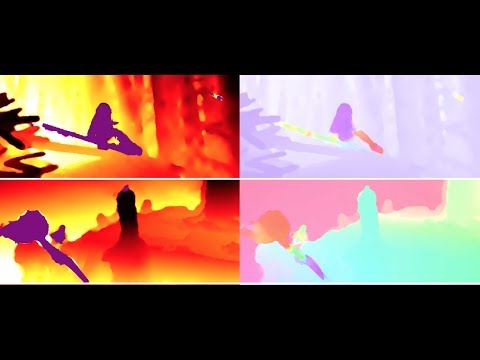
\includegraphics[width=0.8\textwidth]{docs/soba/mr-flow1.jpg}
	\end{minipage}}
 \hfill
  \subfloat[Captopn small box]{
	\begin{minipage}[c][1\width]{
	   0.45\textwidth}
	   \centering
	   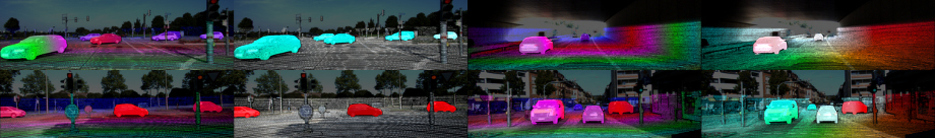
\includegraphics[width=0.8\textwidth]{docs/soba/mr-flow2.jpg}
	\end{minipage}}
 \hfill

\caption{Caption of entire figure}
\end{figure}



\bibliographystyle{plain}
\bibliography{docs/soba/soba}

\end{document}
